% =============================================================================
%  HW03 PRESENTATION --- 8-minute Executive Pitch
%  Sushi Preference in Japan: A Discrete Choice Analysis
%  Universidad de Concepci\'on, Dept. Ingenier\'ia Industrial
% =============================================================================
\documentclass[10pt,aspectratio=169]{beamer}

% --- theme ---
\usetheme{metropolis}
\usecolortheme{default}
\setbeamertemplate{footline}[frame number]
\setbeamertemplate{navigation symbols}{}

% --- packages ---
\usepackage[utf8]{inputenc}
\usepackage[T1]{fontenc}
\usepackage{booktabs}
\usepackage{graphicx}
\usepackage{amsmath,amssymb}
\usepackage{multirow}

% --- paths ---
\graphicspath{{figures/}{Imagenes/}}

% --- info ---
\title{Sushi Preference in Japan:\\A Discrete Choice Analysis}
\subtitle{Understanding Consumer Behavior Through DCM --- HW03}
\author{Mat\'ias Arriagada R. \and Vicente So\~nez I.}
\date{July 2026}
\institute{Universidad de Concepci\'on --- Dept.\ Ingenier\'ia Industrial}
\titlegraphic{\hfill
\includegraphics[height=1.4cm]{logo_dii.png}}

\begin{document}

% =============================================================================
% SLIDE 1 — Title
% =============================================================================
\begin{frame}
  \titlepage
\end{frame}

% =============================================================================
% SLIDE 2 — Research Question + Data
% =============================================================================
\begin{frame}{What Drives Sushi Choice?}
  \begin{columns}[T]
    \column{0.48\textwidth}
    \textbf{Research Question}
    \begin{itemize}
      \item How do price, oiliness, and availability explain sushi preference?
      \item Do age and East/West region moderate taste for oiliness?
      \item Can we predict substitution \& market scenarios?
    \end{itemize}
    \vspace{6pt}
    \textbf{Data: SUSHI Dataset}
    \begin{itemize}
      \item 5,000 Japanese consumers (Kamishima, 2003)
      \item \textbf{Set A}: 10 items, full ranking (used throughout)
      \item Attributes: price, oiliness, freq.\ sold
      \item Demographics: age, gender, 12 regions
    \end{itemize}

    \column{0.48\textwidth}
    \vspace{-8pt}
    \begin{figure}
      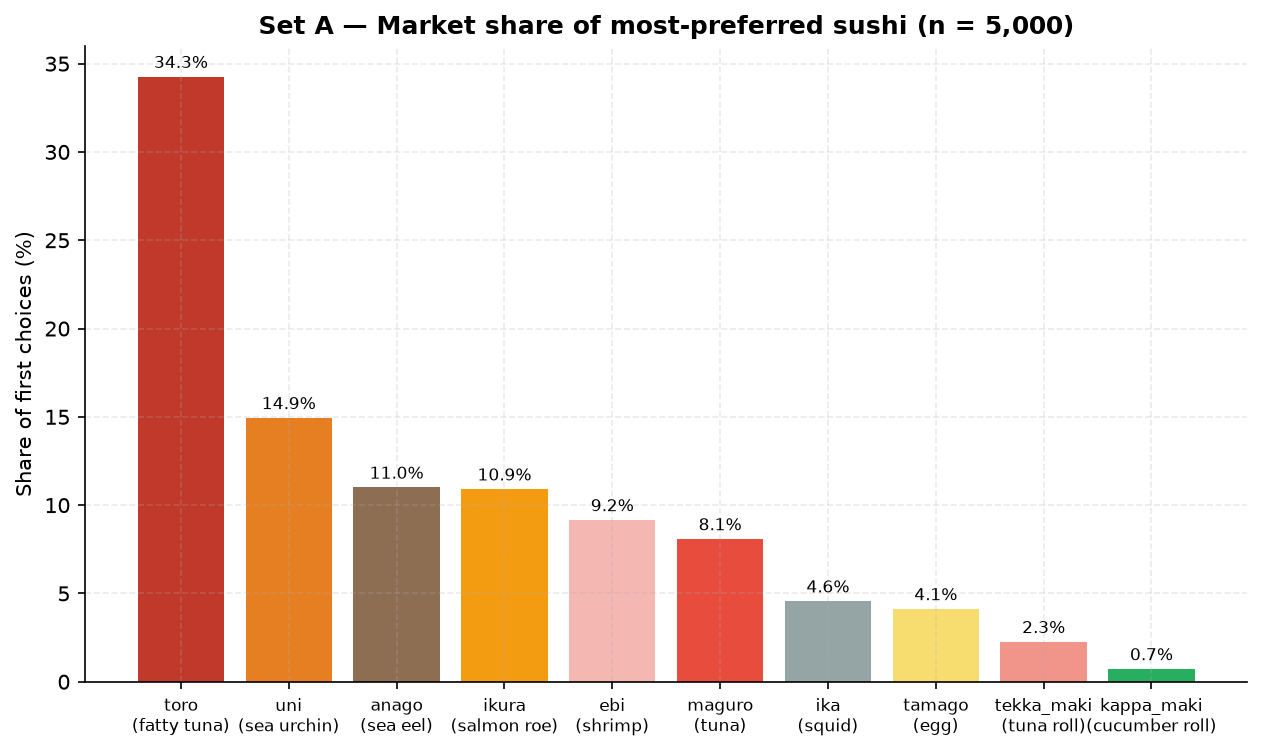
\includegraphics[width=\textwidth]{choice_shares_setA.png}
      \caption*{\footnotesize Toro dominates (34.3\%). Uni, anago, ikura follow.}
    \end{figure}
  \end{columns}
\end{frame}

% =============================================================================
% SLIDE 3 — Identification Challenge
% =============================================================================
\begin{frame}{The Identification Challenge}
  \begin{alertblock}{Critical Design Property}
    Price, oiliness, and freq\_sold are \textbf{constant per item} ---
    all 5,000 users see the same values.\\[4pt]
    $\Rightarrow$ \textbf{ASCs and attribute betas cannot coexist} in one specification
    (perfect collinearity).
  \end{alertblock}

  \vspace{6pt}
  \textbf{Solution}: nested chain of models with LR tests

  \begin{center}
    \begin{tabular}{c c c}
      \textbf{MNL-attributes} (3 betas) & $\subset$ & \textbf{MNL-ASC} (9 ASCs) \\[4pt]
      ``How much do & & ``What do the \\
      attributes explain?'' & & attributes \emph{miss}?'' \\[8pt]
      \multicolumn{3}{c}{\textbf{$\downarrow$ LR test}} \\[4pt]
      \multicolumn{3}{c}{\textbf{M1} (9 ASCs + demographic interactions)} \\[4pt]
      \multicolumn{3}{c}{``Who deviates from the average?''}
    \end{tabular}
  \end{center}
  \vspace{4pt}
  \footnotesize The three headline models are \textbf{M1} (interactions),
  \textbf{M2} (Nested Logit) and \textbf{M3} (Latent Class); the two baselines
  above only anchor the LR chain.
\end{frame}

% =============================================================================
% SLIDE 4 — M3 Results (Star: Age $\times$ Oil)
% =============================================================================
\begin{frame}{M1 — Preferred Model: Age Loves Oil}
  \begin{columns}[T]
    \column{0.52\textwidth}
    \textbf{Specification}
    \begin{equation*}
      U_{nj} = \text{ASC}_j
        + \beta_{p\times w} \cdot \text{price}_j \cdot \text{west}_n
        + \beta_{o\times a} \cdot \text{oil}_j \cdot \text{age}_n
        + \beta_{o\times w} \cdot \text{oil}_j \cdot \text{west}_n
    \end{equation*}

    \vspace{4pt}
    \begin{table}
      \begin{tabular}{lrr}
        \toprule
        Interaction & Coef. & $z$ \\
        \midrule
        $\beta_{\text{price}\times\text{west}}$ & $-0.066$ & $-1.46$ \\
        $\boldsymbol{\beta_{\text{oil}\times\text{age}}}$ & \textbf{+0.089} & \textbf{5.20} \\
        $\beta_{\text{oil}\times\text{west}}$  & $-0.058$ & $-0.86$ \\
        \bottomrule
      \end{tabular}
    \end{table}

    \vspace{2pt}
    \footnotesize LL = $-9{,}733$\;\; $\rho^2 = 0.155$\;\; LR vs MNL-ASC: $p = 10^{-9}$

    \column{0.44\textwidth}
    \begin{figure}
      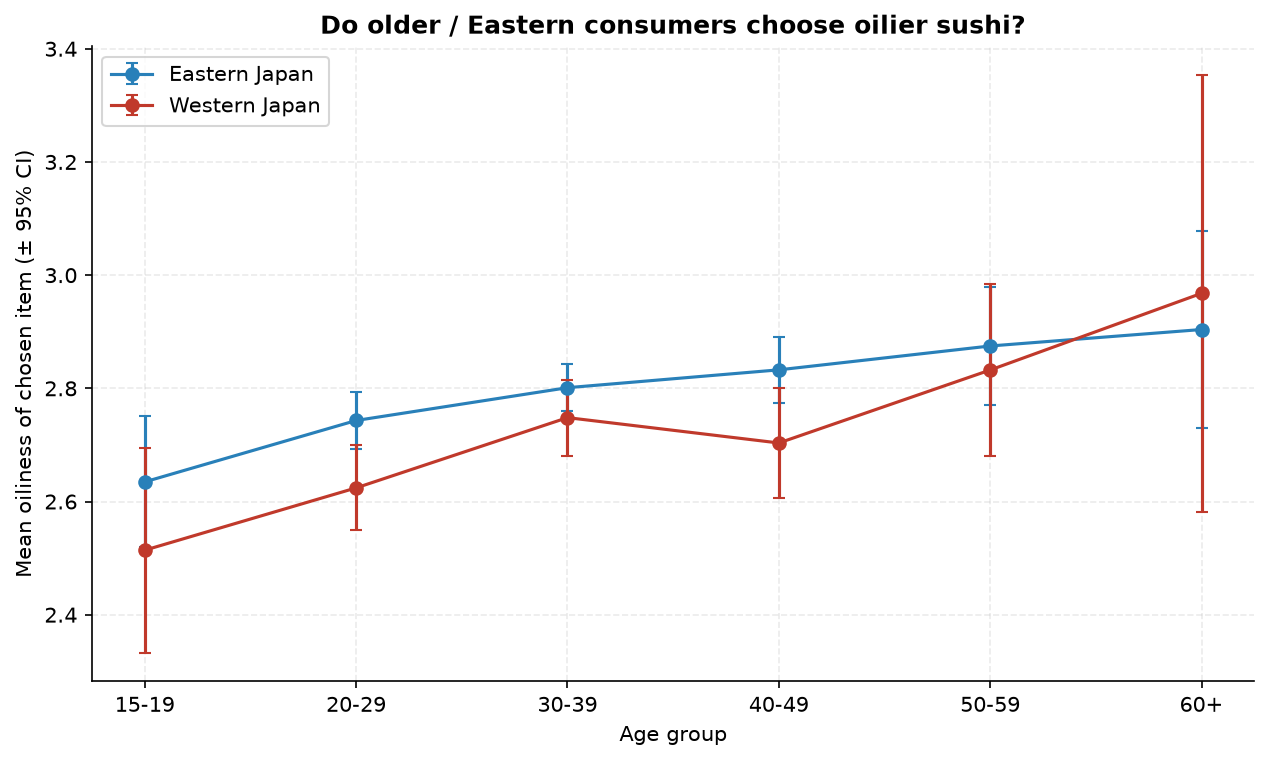
\includegraphics[width=\textwidth]{oiliness_by_eastwest.png}
      \caption*{\footnotesize Older Eastern consumers choose the oiliest sushi.}
    \end{figure}
  \end{columns}

  \vspace{4pt}
  \begin{block}{Bottom line}
    Each step up in age group adds $+0.089$ utils per unit of oiliness ---
    \textbf{older consumers consistently prefer richer, fattier sushi}.
  \end{block}
\end{frame}

% =============================================================================
% SLIDE 5 — East—West Heterogeneity
% =============================================================================
\begin{frame}{East vs.\ West Japan: A Measurable Divide}
  \begin{columns}[T]
    \column{0.45\textwidth}
    \textbf{Individual interactions: not significant}

    Both $\beta_{\text{price}\times\text{west}}$ and $\beta_{\text{oil}\times\text{west}}$
    have $|z| < 1.96$.

    \vspace{8pt}
    \textbf{But joint LR test: $p = 0.0004$}

    The East--West gap is \emph{real} but price and oiliness are too collinear
    ($\rho = 0.82$) to separate cleanly.

    \column{0.51\textwidth}
    \begin{figure}
      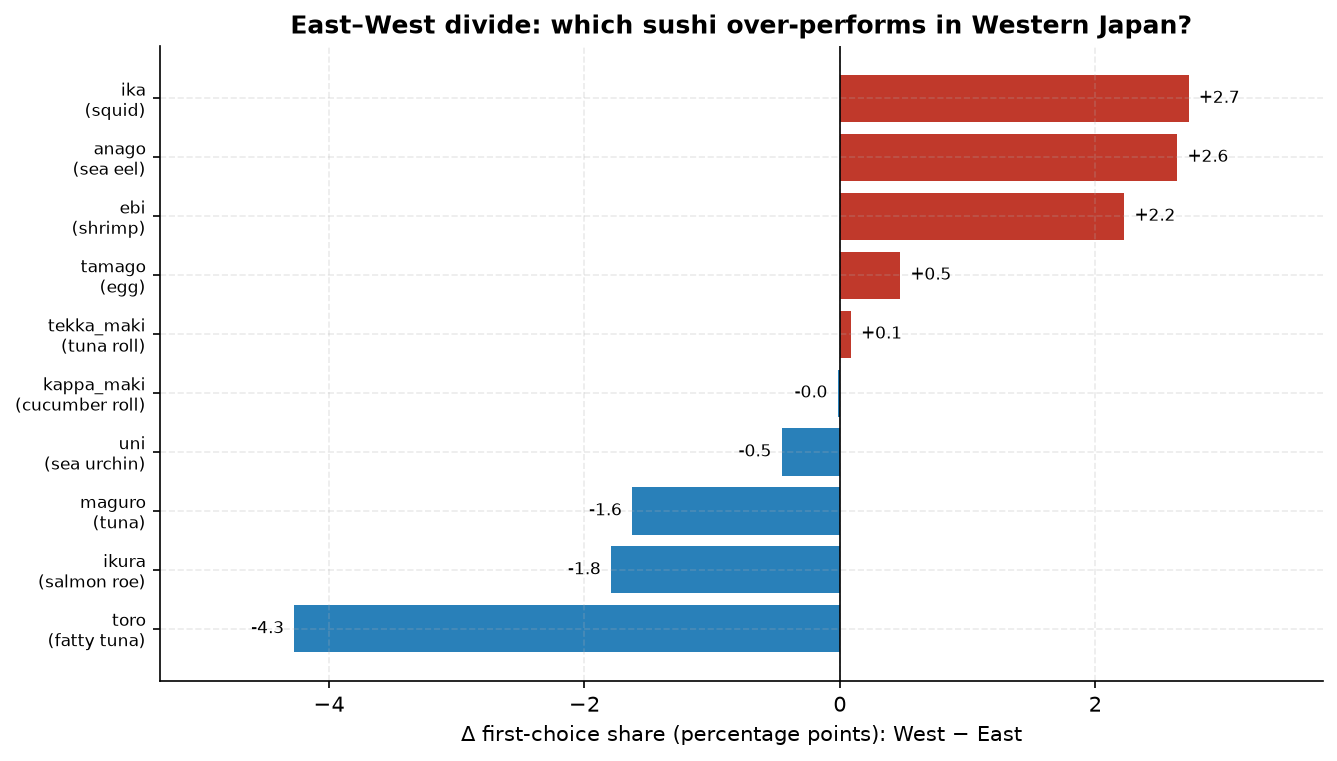
\includegraphics[width=\textwidth]{eastwest_preferences.png}
      \caption*{\footnotesize Systematic East--West differences in choice shares.}
    \end{figure}
  \end{columns}

  \vspace{4pt}
  \begin{exampleblock}{Why it matters}
    The README of the original dataset \emph{predicts} this East--West divide.
    Our model \emph{measures} it, but the attributes' collinearity prevents
    pinpointing the exact channel (price sensitivity vs.\ oiliness aversion).
  \end{exampleblock}
\end{frame}

% =============================================================================
% SLIDE 6 — Nested Logit (IIA Rejected)
% =============================================================================
\begin{frame}{M2 — Nested Logit Rejects IIA}
  \begin{columns}[T]
    \column{0.45\textwidth}
    \textbf{Exploded ranking (ranks 1--3)}

    Each user contributes 3 pseudo-choices:
    \begin{itemize}
      \item Stage 1: all 10 items available
      \item Stage 2: 9 items (rank 1 removed)
      \item Stage 3: 8 items (ranks 1--2 removed)
    \end{itemize}
    $\Rightarrow$ 15,000 pseudo-observations

    \vspace{6pt}
    \textbf{Three nests by ingredient}
    \begin{enumerate}
      \item \texttt{akami}: maguro, toro, tekka\_maki
      \item \texttt{seafood\_other}: ebi, anago, ika, uni, ikura
      \item \texttt{non\_seafood}: tamago, kappa\_maki
    \end{enumerate}

    \column{0.51\textwidth}
    \begin{table}
      \begin{tabular}{lrr}
        \toprule
        $\lambda$ parameter & Estimate & $t$ vs.\ 1 \\
        \midrule
        $\boldsymbol{\lambda_{\text{akami}}}$            & \textbf{0.323} & $-26.1$ \\
        $\boldsymbol{\lambda_{\text{seafood\_other}}}$   & \textbf{0.342} & $-6.9$ \\
        $\lambda_{\text{non\_seafood}}$                  & 1.000 & (fixed) \\
        \bottomrule
      \end{tabular}
    \end{table}

    \vspace{2pt}
    \footnotesize LR vs MNL-exploded = 573.5, $p \approx 0$\\
    \footnotesize A free $\lambda_{\text{non\_seafood}}$ hits the $\lambda \to 0$
    boundary (degenerate 2-item nest), so it is fixed at 1.

    \vspace{6pt}
    \begin{center}
      \Large \textbf{$\lambda < 1$ in both free nests}\\[4pt]
      \normalsize Substitution is much stronger\\
      within nests than MNL predicts.
    \end{center}
  \end{columns}
\end{frame}

% =============================================================================
% SLIDE 6b — Latent Class: who are the segments?
% =============================================================================
\begin{frame}{M3 — Three Latent Consumer Segments (LC-MNL, Apollo)}
  \textbf{Latent Class MNL} on the exploded ranking; class membership driven by
  age, region, gender, migration. BIC selects \textbf{3 classes}
  (LL $-28{,}514$ vs.\ $-29{,}446$ with 1 class).

  \vspace{4pt}
  \begin{table}
    \small
    \begin{tabular}{lccc}
      \toprule
      & \textbf{Premium gourmet} & \textbf{Light taste} & \textbf{Tuna fanatic} \\
      \midrule
      Share            & 33.7\% & 31.3\% & 34.9\% \\
      Signature items  & uni, ikura, toro & ebi (all else $<$ 0) & toro, maguro, tekka \\
      Rejects          & egg, rolls & \textbf{uni} ($-2.2$) & cucumber roll \\
      Profile          & oldest, 51\% F & youngest, West, 64\% F & most male, East \\
      \bottomrule
    \end{tabular}
  \end{table}

  \vspace{6pt}
  \begin{block}{Convergent evidence}
    The ``tuna fanatic'' class \emph{is} the akami nest seen as a person type.
    And uni's polarization (loved by gourmets at $+1.9$, rejected by the light
    class at $-2.2$) explains the rank-stability drift found in robustness checks.
  \end{block}
\end{frame}

% =============================================================================
% SLIDE 7 — Scenario A: Toro Shock
% =============================================================================
\begin{frame}{Scenario A: What If Toro Becomes Scarce?}
  \textbf{Intervention:} Toro price $+40\%$ (bluefin tuna quota reduction)
  \vspace{4pt}

  \begin{figure}
    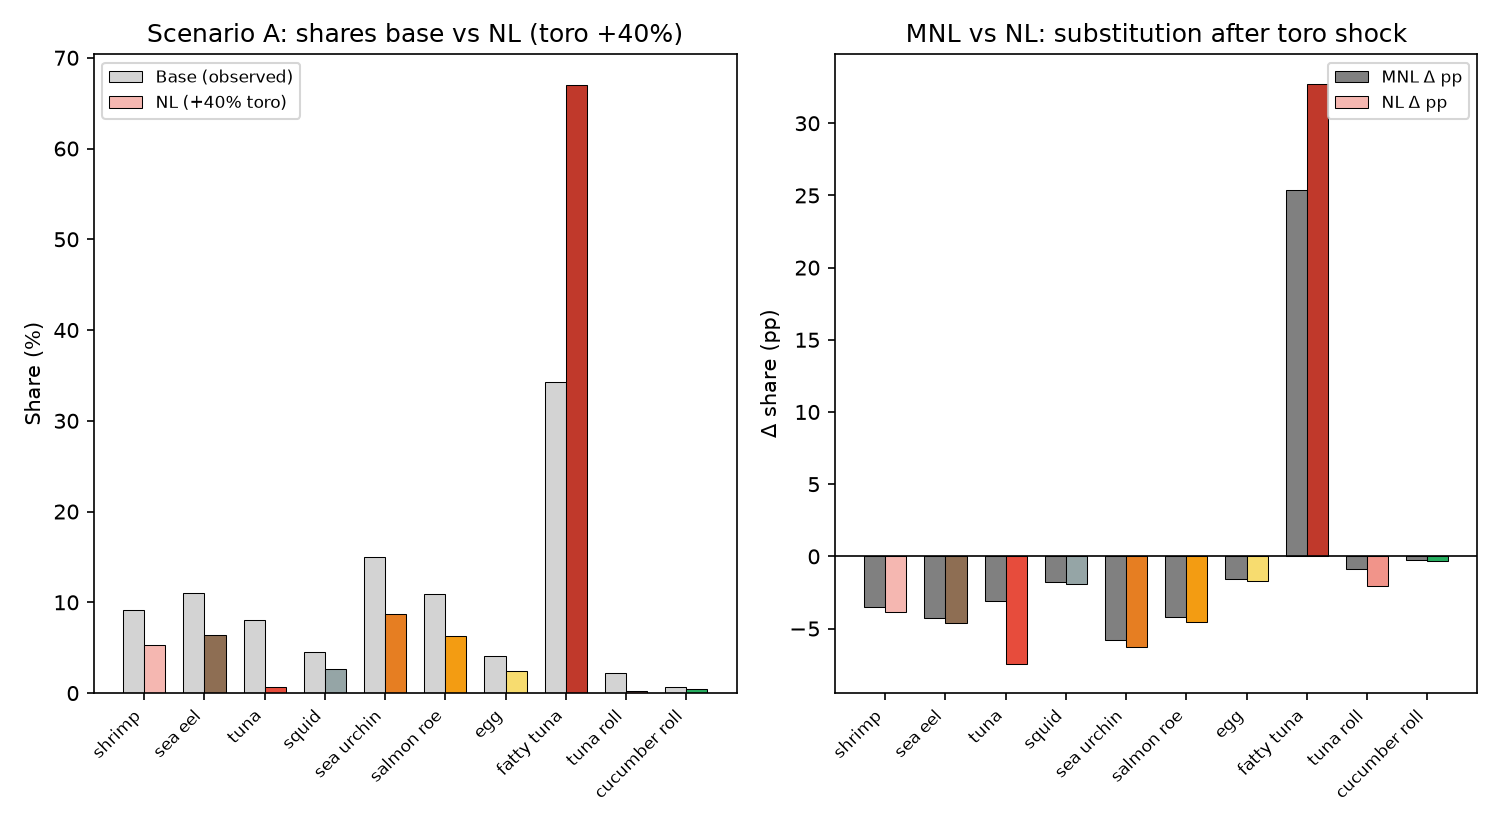
\includegraphics[width=0.88\textwidth]{scenario_A_nl_mnl.png}
  \end{figure}

  \begin{block}{The MNL-NL gap IS the finding}
    \begin{itemize}
      \item MNL: all cross-elasticities identical ($-$0.97) --- IIA in action
      \item NL: maguro and tekka\_maki (same nest) lose \textbf{far more} share
      \item $\lambda_{\text{akami}} = 0.33 \;\Rightarrow\;$ Within-nest substitution
            is 3$\times$ stronger than MNL assumes
    \end{itemize}
  \end{block}
\end{frame}

% =============================================================================
% SLIDE 8 — Scenario B: Healthy Promotion
% =============================================================================
\begin{frame}{Scenario B: Can Price Make Sushi Healthier?}
  \begin{columns}[T]
    \column{0.48\textwidth}
    \textbf{Intervention: kappa-maki (cucumber roll)}
    \begin{itemize}
      \item $-30\%$ price
      \item availability \texttt{freq\_sold} $0.40 \to 0.88$ (p75)
      \item heterogeneity via M1 age $\times$ West
    \end{itemize}

    \vspace{6pt}
    \begin{table}\small
      \begin{tabular}{lccc}
        \toprule
        Segment & Base \% & CF \% & $\Delta$ pp \\
        \midrule
        Young East & 0.52 & 1.23 & +0.71 \\
        Young West & 0.70 & 1.65 & \textbf{+0.95} \\
        \textbf{All} & \textbf{0.52} & \textbf{1.23} & \textbf{+0.71} \\
        \bottomrule
      \end{tabular}
    \end{table}

    \column{0.48\textwidth}
    \begin{figure}
      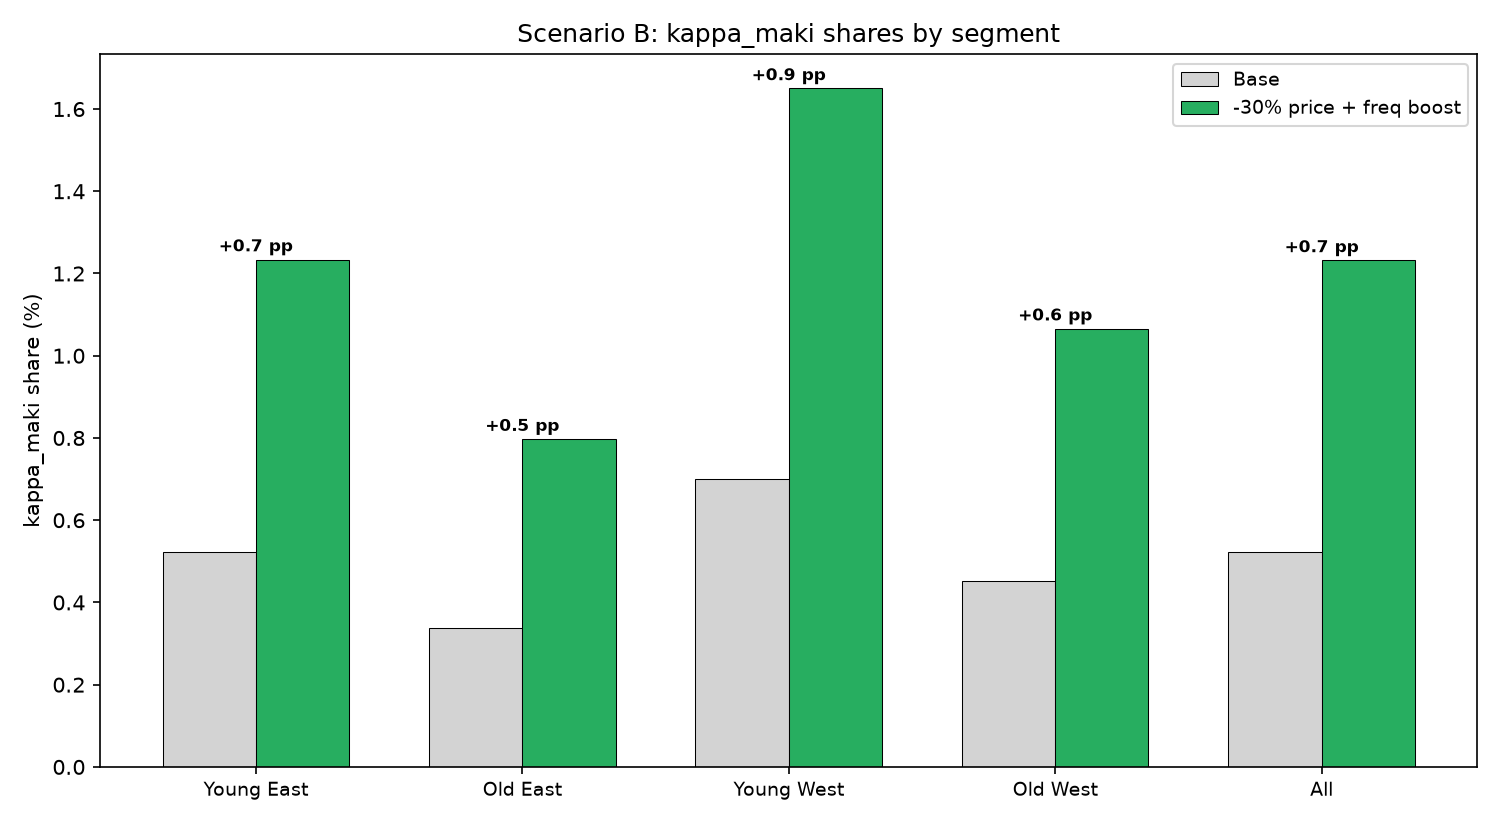
\includegraphics[width=\textwidth]{scenario_B_segments.png}
    \end{figure}
  \end{columns}

  \vspace{4pt}
  \begin{exampleblock}{Health-policy insight}
    Even $-30\%$ price + a big availability push lifts the healthiest item only
    from 0.5\% to 1.2\%. And since $\beta_{\text{price}} > 0$, the \emph{discount
    hurts} --- the gain comes entirely from availability ($\beta_{\text{freq}}$).
  \end{exampleblock}
\end{frame}

% =============================================================================
% SLIDE 9 — Recommendations
% =============================================================================
\begin{frame}{Strategic Recommendations}
  \begin{columns}[T]
    \column{0.48\textwidth}
    \textbf{For Industry}
    \begin{enumerate}
      \item \textbf{Menu design:} When toro sells out, stock up on maguro
            and tekka\_maki --- not proportional restocking (M2, $\lambda_{\text{akami}}=0.32$).
      \item \textbf{Regional targeting:} Premium fatty items $\rightarrow$
            older Eastern consumers. Light items $\rightarrow$ younger Western consumers.
      \item \textbf{Segment offers:} Three latent segments (gourmet / light /
            tuna-fanatic) are addressable by age, gender and region (M3).
    \end{enumerate}

    \column{0.48\textwidth}
    \textbf{For Public Policy}
    \begin{enumerate}
      \item \textbf{Don't subsidize healthy sushi:} $\beta_{\text{price}} > 0$
            means cheaper = lower perceived quality.
      \item \textbf{Boost availability instead:} $\beta_{\text{freq\_sold}} = +2.17$
            is the largest coefficient. Make healthier options visible.
      \item \textbf{Reframe, don't discount:} Market light sushi as premium
            craftsmanship, not ``cheap healthy alternative.''
      \item \textbf{Cultural preservation:} Regional taste differences are real
            --- leverage identity, not price.
    \end{enumerate}
  \end{columns}

  \vspace{8pt}
  \begin{center}
    \small\textit{Full details in the written report (\S D.1--D.3).}
  \end{center}
\end{frame}

% =============================================================================
% SLIDE 10 — Limitations + Thank You
% =============================================================================
\begin{frame}{Limitations \& Next Steps}

  \begin{alertblock}{Key Caveats}
    \begin{itemize}
      \item $\beta_{\text{price}} > 0$: price signals quality in this survey;
            WTP and price scenarios are \textbf{not monetary}.
      \item $\text{corr}(\text{price}, \text{oiliness}) = 0.82$ in Set A:
            multicollinearity inflates SEs, so price scenarios are read qualitatively.
      \item Rank explosion assumes stable preferences across ranking stages.
      \item Fixed 10-item choice set: strong LR tests, but no generalisation
            beyond Set A.
    \end{itemize}
  \end{alertblock}

  \vspace{4pt}
  \textbf{Validation \& future work}
  \begin{itemize}
    \item Apollo (R) cross-validation \textbf{completed}: log-likelihoods match
          the Python engine to $\leq 0.01$ across all models.
    \item Latent Class (3 segments) estimated; a continuous Mixed Logit could
          capture residual within-class heterogeneity.
    \item Revealed-preference data for interpretable price effects.
  \end{itemize}

  \vspace{8pt}
  \begin{center}
    {\Large \textbf{Thank you}}\\[8pt]
    \footnotesize
    Code, data, and full report at:
    \fbox{\textbf{PENDING: insert shared-folder link before submission}}\\[4pt]
    Questions?
  \end{center}
\end{frame}

\end{document}
